\documentclass{article}

\usepackage{generalsnips}
\usepackage{calculussnips}
\usepackage{programmingsnips}
\usepackage[margin = 1in]{geometry}
\usepackage{pdfpages}
\usepackage[spanish]{babel}
\usepackage{amsmath}
\usepackage{amsthm}
\usepackage[utf8]{inputenc}
\usepackage{titlesec}
\usepackage{xpatch}
\usepackage{fancyhdr}
\usepackage{tikz}
\usepackage{hyperref}
\usepackage{minted}
\usepackage{amssymb}
\usepackage{float}

\darktheme
\title{Algoritmo Dijstrka - Applicación 2}
\date{15 de noviembre 2020} % , 05:33PM
\author{David Corzo \& Jean Pierre Mejicanos}

\begin{document}
\maketitle
%%%%%%%%%%%%%%%%%%%%%%%%%%%%%%%%%%%%%%%%%%%%%%%%%%%%%%%%%%%%%%%%%%%%%%%%%%%%%%%%%%%%%%%%%%%%%%%%%%%%%%%%%%%%%%%%%%%%%%%%%%%%%%%%%%%%%%%%%%%%%%

\section{Implementación de algoritmo Dijkstra}
En el método \verb|dijktra| se encuentra la implementación del algoritmo Dijsktra. En el método \verb|dibujar_grafica| se encuentra la implementación para graficar el grafo ingresado.
\inputcode{py}{./dijkstrafinal.py}
\begin{minted}[autogobble]{py}
# Output:
#     The path between 1 to 6
#     1->2->3->5->4->6
\end{minted}
Y el output gráfico que se aprecia a continuación: 
\begin{figure}[H]
    \centering
    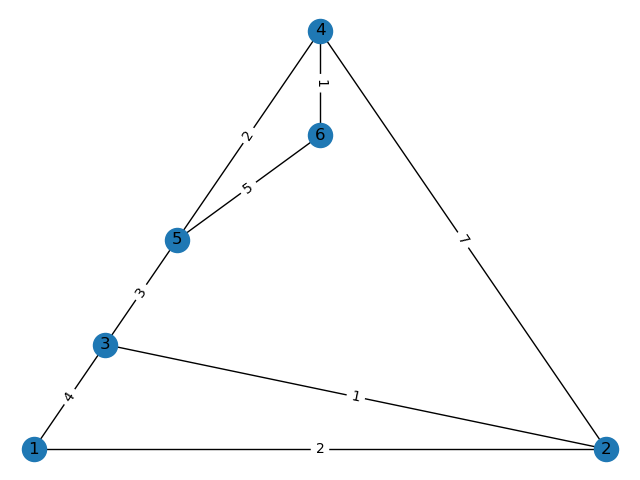
\includegraphics[width=0.7\textwidth]{grafo0}
    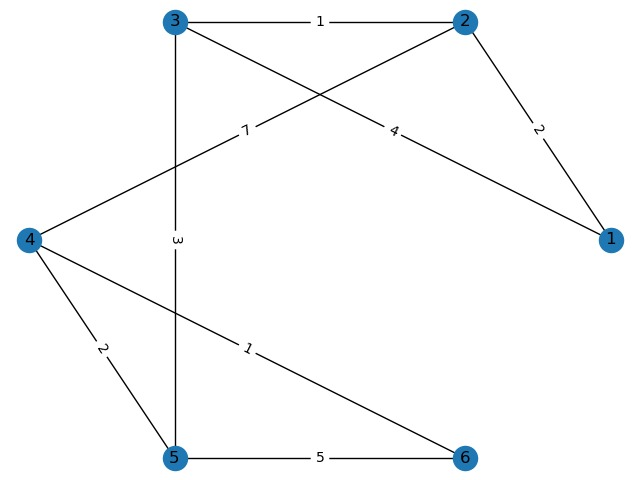
\includegraphics[width=0.7\textwidth]{grafo1.jpeg}
    \caption{Grafo ingresado}
\end{figure}


\section{Análisis de complejidad del algoritmo}
A continuación presentamos los casos de atención en el algoritmo.
\begin{itemize}
    \item Para preparar los nodos tomamos $n$, se puede ver en el fragmento de algoritmo a continuación. 
        \begin{minted}[autogobble]{py}
            for node in self.grafo: # n
                self.pesos[node] = float("inf") # 1*n
                self.camino[node] = None # 1*n
                self.nodos_restantes.append(node) # 1*n
        \end{minted}
        \begin{itemize}
            \item Observamos que la complejidad del peor escenario de este pedazo de código es $O(n)$ 
        \end{itemize}
    
    \item Esta sección de código a continuación fabrica la matriz de adyacencia pertinente al algoritmo Dijkstra.
        \begin{minted}[autogobble]{py}
            while len(self.nodos_restantes) != 0: # n
                llave_minima = min(self.nodos_restantes) # n*n
                nodo_actual = llave_minima # 1*n
                self.nodos_restantes.remove(nodo_actual) # 1*n
                
                for nodo in self.grafo[nodo_actual]: # n*n
                    alternativa = self.grafo[nodo_actual][nodo] + self.pesos[nodo_actual] # 1*n*n
                    if self.pesos[nodo] > alternativa: # 1*n*n
                        self.pesos[nodo] = alternativa 
                        self.camino[nodo] = nodo_actual
        \end{minted}
        \begin{itemize}
            \item Observamos que la complejidad del peor escenario de este pedazo código es $O(n^2)$ 
        \end{itemize}
    
    \item Para determinar qué camino tomar (ya fabricada la matriz de adyacencia) tomamos este código a continuación:
        \begin{minted}[autogobble]{py}
            while True: # n
                nodo_destino = self.camino[nodo_destino] # 1*n 
                if nodo_destino is None: 
                    break
                order.insert(0,nodo_destino) # 1*n
        \end{minted}
        \begin{itemize}
            \item Observamos que la complejidad del peor caso de este código es: $O(n)$ 
        \end{itemize}
\end{itemize}

$\therefore$ Por lo anterior se puede afirmar que la complejidad de la implementación de este código Dijkstra es $O(n^2)$.




%%%%%%%%%%%%%%%%%%%%%%%%%%%%%%%%%%%%%%%%%%%%%%%%%%%%%%%%%%%%%%%%%%%%%%%%%%%%%%%%%%%%%%%%%%%%%%%%%%%%%%%%%%%%%%%%%%%%%%%%%%%%%%%%%%%%%%%%%%%%%%
\end{document}

